\chapter{Verkkojen perusteet}

\section{Verkkojen käsitteitä}

Verkko on tietorakenne, joka muodostuu \emph{solmuista} ja
niitä yhdistävistä \emph{kaarista}.
Merkitsemme tässä kirjassa verkon solmujen
määrää kirjaimella $n$ ja verkon kaarten määrää
kirjaimella $m$.
Lisäksi numeroimme yleensä verkon solmut kokonaisluvuin
$1,2,\dots,n$.

Sanomme, että kaksi solmua ovat \emph{vierekkäin} verkossa,
jos niiden välillä on kaari.
Solmun \emph{naapureja} ovat kaikki solmut,
joihin se on yhteydessä kaarella,
ja solmun \emph{aste} on sen naapureiden määrä.
Verkossa oleva \emph{polku} tarkoittaa reittiä
tietystä solmusta toiseen kulkemalla kaaria pitkin.

Kuvassa \ref{fig:veresi} on esimerkkinä verkko,
jossa on 5 solmua ja 7 kaarta.
Solmun 2 aste on 3,
koska sen naapurit ovat solmut 1, 4 ja 5.
Voimme kulkea solmusta 1 solmuun 5 monella tavalla:
mahdollisia polkuja ovat esimerkiksi
$1 \rightarrow 2 \rightarrow 5$ ja
$1 \rightarrow 3 \rightarrow 4 \rightarrow 5$.

\begin{figure}
\center
\begin{center}
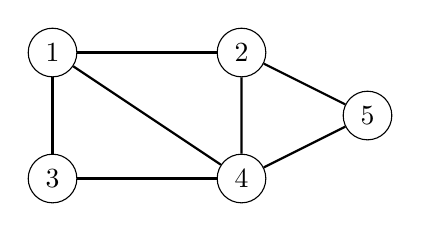
\begin{tikzpicture}[scale=0.8]
\node[draw, circle] (1) at (1,3) {$1$};
\node[draw, circle] (2) at (4,3) {$2$};
\node[draw, circle] (3) at (1,1) {$3$};
\node[draw, circle] (4) at (4,1) {$4$};
\node[draw, circle] (5) at (6,2) {$5$};

\path[draw,thick,-] (1) -- (2);
\path[draw,thick,-] (1) -- (3);
\path[draw,thick,-] (1) -- (4);
\path[draw,thick,-] (3) -- (4);
\path[draw,thick,-] (2) -- (4);
\path[draw,thick,-] (2) -- (5);
\path[draw,thick,-] (4) -- (5);
\end{tikzpicture}
\end{center}
\caption{Verkko, jossa on 5 solmua ja 7 kaarta.}
\label{fig:veresi}
\end{figure}

Verkko on \emph{yhtenäinen}, jos minkä tahansa
kahden solmun välillä on polku.
Esimerkiksi kuvan \ref{fig:veresi} verkko on yhtenäinen.
Jos verkko ei ole yhtenäinen, voimme tarkastella
sen yhtenäisiä \emph{komponentteja}.
Esimerkiksi kuvan \ref{fig:veryht} verkko ei ole yhtenäinen,
ja sen komponentit ovat $\{1,3\}$ ja $\{2,4,5\}$.

\begin{figure}
\center
\begin{center}
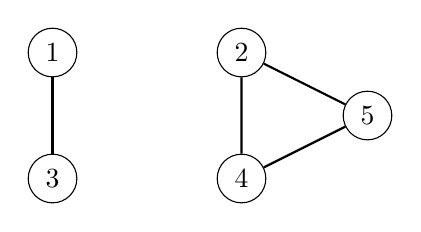
\begin{tikzpicture}[scale=0.8]
\node[draw, circle] (1) at (1,3) {$1$};
\node[draw, circle] (2) at (4,3) {$2$};
\node[draw, circle] (3) at (1,1) {$3$};
\node[draw, circle] (4) at (4,1) {$4$};
\node[draw, circle] (5) at (6,2) {$5$};

\path[draw,thick,-] (1) -- (3);
\path[draw,thick,-] (2) -- (4);
\path[draw,thick,-] (2) -- (5);
\path[draw,thick,-] (4) -- (5);
\end{tikzpicture}
\end{center}
\caption{Verkon yhtenäiset komponentit ovat $\{1,3\}$ ja $\{2,4,5\}$.}
\label{fig:veryht}
\end{figure}

Verkossa oleva \emph{sykli} on polku, jonka ensimmäinen ja viimeinen
solmu on sama.
Esimerkiksi verkossa \ref{fig:veresi} on sykli
$1 \rightarrow 4 \rightarrow 3 \rightarrow 1$.
Verkko on \emph{syklitön}, jos siinä ei ole yhtään sykliä.
Verkko on \emph{puu}, jos se on yhtenäinen ja syklitön.
Puussa kaarten määrä on aina yhden pienempi kuin solmujen määrä.
Esimerkiksi kuvassa \ref{fig:verpuu} on puu, jossa on 5 solmua ja 4 kaarta.

\begin{figure}
\center
\begin{center}
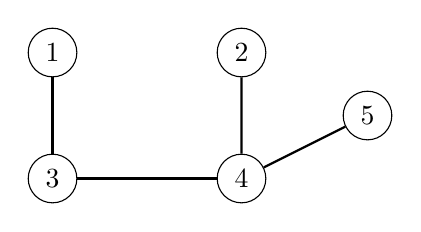
\begin{tikzpicture}[scale=0.8]
\node[draw, circle] (1) at (1,3) {$1$};
\node[draw, circle] (2) at (4,3) {$2$};
\node[draw, circle] (3) at (1,1) {$3$};
\node[draw, circle] (4) at (4,1) {$4$};
\node[draw, circle] (5) at (6,2) {$5$};

\path[draw,thick,-] (1) -- (3);
\path[draw,thick,-] (3) -- (4);
\path[draw,thick,-] (2) -- (4);
\path[draw,thick,-] (4) -- (5);
\end{tikzpicture}
\end{center}
\caption{Puu, jossa on 5 solmua ja 4 kaarta.}
\label{fig:verpuu}
\end{figure}

Verkko on \emph{suunnattu}, jos kaarilla on merkityt suunnat,
joiden mukaisesti niitä on kuljettava.
Kuvassa \ref{fig:versuu} on esimerkkinä suunnattu verkko.
Esimerkiksi voimme kulkea solmusta 1 solmuun 5
polkua $1 \rightarrow 2 \rightarrow 5$,
mutta emme voi kulkea solmusta 5 solmuun 1.

\begin{figure}
\center
\begin{center}
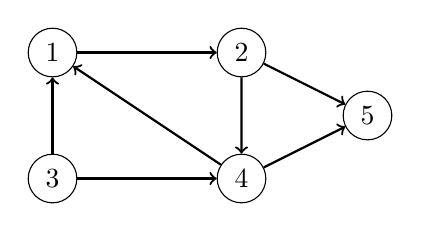
\begin{tikzpicture}[scale=0.8]
\node[draw, circle] (1) at (1,3) {$1$};
\node[draw, circle] (2) at (4,3) {$2$};
\node[draw, circle] (3) at (1,1) {$3$};
\node[draw, circle] (4) at (4,1) {$4$};
\node[draw, circle] (5) at (6,2) {$5$};

\path[draw,thick,->] (1) -- (2);
\path[draw,thick,<-] (1) -- (3);
\path[draw,thick,<-] (1) -- (4);
\path[draw,thick,->] (3) -- (4);
\path[draw,thick,->] (2) -- (4);
\path[draw,thick,->] (2) -- (5);
\path[draw,thick,->] (4) -- (5);
\end{tikzpicture}
\end{center}
\caption{Suunnattu verkko.}
\label{fig:versuu}
\end{figure}

Suunnattu verkko on \emph{vahvasti yhtenäinen},
jos verkossa on polku mistä tahansa solmusta
mihin tahansa solmuun.
Esimerkiksi kuvan \ref{fig:versuu} verkko ei
ole vahvasti yhtenäinen,
koska emme voi kulkea solmusta 5 solmuun 1.
Jos verkko ei ole vahvasti yhtenäinen,
voimme jakaa sen vahvasti yhtenäisiin komponentteihin.
Esimerkiksi kuvan \ref{fig:versuu} verkossa
vahvasti yhtenäiset komponentit ovat $\{1,2,4\}$, $\{3\}$ ja $\{5\}$.

Suunnatussa verkossa solmun \emph{lähtöaste} on
solmusta lähtevien kaarten määrä ja solmun \emph{tuloaste}
on solmuun tulevien kaarten määrä.
Esimerkiksi kuvan \ref{fig:versuu} verkossa
solmun 2 lähtöaste on 2 ja tuloaste on 1.

Verkko on \emph{painotettu}, jos sen kaarille on asetettu painot.
Usein painot kuvaavat kaarien pituuksia, ja polun pituus
on siinä olevien painojen summa.
Kuvassa \ref{fig:verpai} on esimerkki painotetusta verkosta.
Esimerkiksi polun $1 \rightarrow 3 \rightarrow 4 \rightarrow 5$
pituus on $2+4+3=9$.

\begin{figure}
\center
\begin{center}
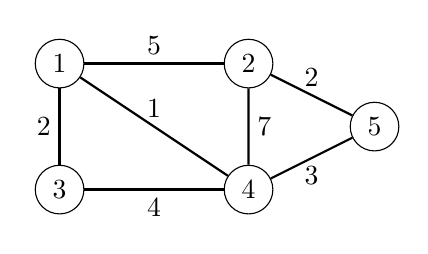
\begin{tikzpicture}[scale=0.8,label distance=-1.5mm]
\node[draw, circle] (1) at (1,3) {$1$};
\node[draw, circle] (2) at (4,3) {$2$};
\node[draw, circle] (3) at (1,1) {$3$};
\node[draw, circle] (4) at (4,1) {$4$};
\node[draw, circle] (5) at (6,2) {$5$};

\path[draw,thick,-] (1) -- node[font=\small,label=above:5] {} (2);
\path[draw,thick,-] (1) -- node[font=\small,label=left:2] {} (3);
\path[draw,thick,-] (1) -- node[font=\small,label=above:1] {} (4);
\path[draw,thick,-] (3) -- node[font=\small,label=below:4] {} (4);
\path[draw,thick,-] (2) -- node[font=\small,label=right:7] {} (4);
\path[draw,thick,-] (2) -- node[font=\small,label=above:2] {} (5);
\path[draw,thick,-] (4) -- node[font=\small,label=below:3] {} (5);
\end{tikzpicture}
\end{center}
\caption{Painotettu verkko.}
\label{fig:verpai}
\end{figure}

Verkko on \emph{kaksijakoinen}, jos voimme värittää sen
solmut kahdella värillä niin, että jokaisella
vierekkäisellä solmulla on eri väri.
Esimerkiksi kuvan \ref{fig:verkak} verkko on kaksijakoinen,
koska voimme värittää solmut 1 ja 4 sinisiksi ja
solmut 2, 3 ja 5 punaisiksi.

\begin{figure}
\center
\begin{center}
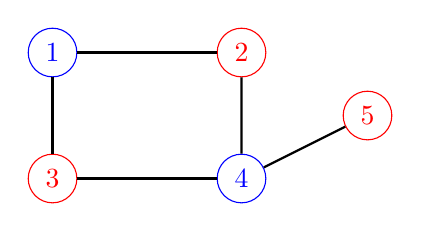
\begin{tikzpicture}[scale=0.8]
\node[draw, circle, color=blue] (1) at (1,3) {$1$};
\node[draw, circle, color=red] (2) at (4,3) {$2$};
\node[draw, circle, color=red] (3) at (1,1) {$3$};
\node[draw, circle, color=blue] (4) at (4,1) {$4$};
\node[draw, circle, color=red] (5) at (6,2) {$5$};

\path[draw,thick,-] (1) -- (2);
\path[draw,thick,-] (1) -- (3);
\path[draw,thick,-] (3) -- (4);
\path[draw,thick,-] (2) -- (4);
\path[draw,thick,-] (4) -- (5);
\end{tikzpicture}
\end{center}
\caption{Kaksijakoinen verkko.}
\label{fig:verkak}
\end{figure}

\section{Verkot ohjelmoinnissa}

Seuraavaksi käymme läpi kaksi tavallista tapaa
käsitellä verkkoa ohjelmoinnissa.
Vieruslistaesityksessä tallennamme jokaiselle
solmulle listan solmuista, joihin siitä pääsee kaarella.
Vierusmatriisiesityksessä taas luomme kaksiulotteisen
taulukon, joka ilmaisee verkossa olevat kaaret.

\subsection{Vieruslistaesitys}

Verkon vieruslistaesityksessä jokaisella solmulla on
\emph{vieruslista}, joka ilmaisee, mihin solmuihin
solmusta lähtee kaari.
Kuvassa \ref{fig:vervil} on esimerkkinä suunnattu verkko
sekä sitä vastaava vieruslistaesitys.

\begin{figure}
\center
\begin{center}
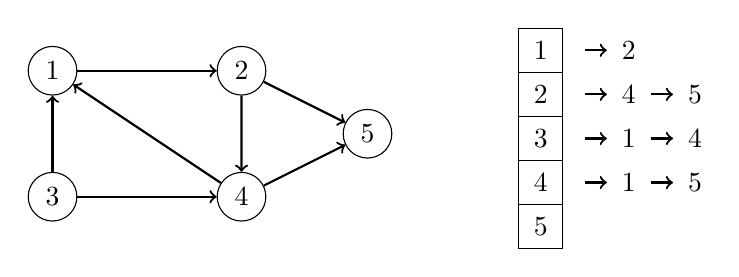
\begin{tikzpicture}[scale=0.8]
\begin{scope}
\node[draw, circle] (1) at (1,3) {$1$};
\node[draw, circle] (2) at (4,3) {$2$};
\node[draw, circle] (3) at (1,1) {$3$};
\node[draw, circle] (4) at (4,1) {$4$};
\node[draw, circle] (5) at (6,2) {$5$};

\path[draw,thick,->] (1) -- (2);
\path[draw,thick,<-] (1) -- (3);
\path[draw,thick,<-] (1) -- (4);
\path[draw,thick,->] (3) -- (4);
\path[draw,thick,->] (2) -- (4);
\path[draw,thick,->] (2) -- (5);
\path[draw,thick,->] (4) -- (5);
\end{scope}
\begin{scope}[scale=0.7,xshift=12cm,yshift=0.25cm]
\draw (0,0) grid (1,5);
\foreach \y/\v in {0/1,1/2,2/3,3/4,4/5} \node at (0.5,4.5-\y) {\v};
\node at (2.5,4.5) {2};
\node at (2.5,3.5) {4};
\node at (4,3.5) {5};
\node at (2.5,2.5) {1};
\node at (4,2.5) {4};
\node at (2.5,1.5) {1};
\node at (4,1.5) {5};
\path[draw,thick,->] (1.5,4.5) -- (2,4.5);
\path[draw,thick,->] (1.5,3.5) -- (2,3.5);
\path[draw,thick,->] (1.5,2.5) -- (2,2.5);
\path[draw,thick,->] (1.5,1.5) -- (2,1.5);
\path[draw,thick,->] (3,3.5) -- (3.5,3.5);
\path[draw,thick,->] (3,2.5) -- (3.5,2.5);
\path[draw,thick,->] (3,1.5) -- (3.5,1.5);
\end{scope}
\end{tikzpicture}
\end{center}
\caption{Verkon vieruslistaesitys.}
\label{fig:vervil}
\end{figure}

Javassa voimme tallentaa verkon vieruslistaesityksen
taulukkona, jonka jokaisessa kohdassa on tietyn
solmun vieruslista.
Seuraava koodi määrittelee tällaisen taulukon:

\begin{code}
ArrayList<Integer>[] verkko = new ArrayList<>[n+1];
\end{code}

Ennen kuin voimme käyttää taulukkoa,
meidän täytyy alustaa jokainen vieruslista:

\begin{code}
for (int i = 1; i <= n; i++) {
    verkko[i] = new ArrayList<>();
}
\end{code}

Tämän jälkeen voimme lisätä kaaret verkkoon näin:

\begin{code}
verkko[1].add(2);
verkko[2].add(4);
verkko[2].add(5);
verkko[3].add(1);
verkko[3].add(4);
verkko[4].add(1);
verkko[4].add(5);
\end{code}

Jos verkko on suuntaamaton, voimme menetellä muuten samoin,
mutta tallennamme kunkin kaaren molempiin suuntiin.
Jos taas verkko on painotettu, voimme tallentaa listaan
sekä kaarten kohdesolmut että painot.

Vieruslistaesitys on yleensä käytännössä hyvä tapa
tallentaa verkko ohjelmoinnissa.
Esityksen etuna on, että voimme selvittää helposti,
mihin solmuihin pääsee kaarta pitkin tietystä solmusta.
Esimerkiksi voimme käydä seuraavasti läpi solmut,
joihin pääsee kaarella solmusta $x$:

\begin{code}
for (Integer u : verkko[x]) {
    // käsittele solmu u
}
\end{code}

\subsection{Vierusmatriisiesitys}

Verkon vierusmatriisiesityksessä luomme $n \times n$ -matriisin
(eli kaksiulotteisen taulukon), joka kuvaa, mitä kaaria verkossa on.
Matriisissa rivin $a$ sarakkeessa $b$ on luku 1,
jos verkossa on kaari solmusta $a$ solmuun $b$,
ja muuten luku 0.
Kuvassa \ref{fig:vervil} on esimerkki verkon
vierusmatriisiesityksestä.

\begin{figure}
\center
\begin{center}
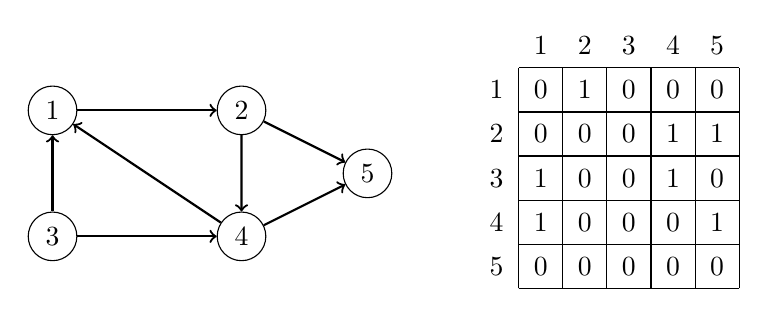
\begin{tikzpicture}[scale=0.8]
\begin{scope}
\node[draw, circle] (1) at (1,3) {$1$};
\node[draw, circle] (2) at (4,3) {$2$};
\node[draw, circle] (3) at (1,1) {$3$};
\node[draw, circle] (4) at (4,1) {$4$};
\node[draw, circle] (5) at (6,2) {$5$};

\path[draw,thick,->] (1) -- (2);
\path[draw,thick,<-] (1) -- (3);
\path[draw,thick,<-] (1) -- (4);
\path[draw,thick,->] (3) -- (4);
\path[draw,thick,->] (2) -- (4);
\path[draw,thick,->] (2) -- (5);
\path[draw,thick,->] (4) -- (5);
\end{scope}
\begin{scope}[scale=0.7,xshift=12cm,yshift=0.25cm]
\draw (0,0) grid (5,5);
\foreach \x in {1,2,3,4,5} \node at (-0.5,5.5-\x) {\x};
\foreach \x in {1,2,3,4,5} \node at (-0.5+\x,5.5) {\x};

\foreach \x/\v in {1/0,2/1,3/0,4/0,5/0} \node at (-0.5+\x,4.5) {\v};
\foreach \x/\v in {1/0,2/0,3/0,4/1,5/1} \node at (-0.5+\x,3.5) {\v};
\foreach \x/\v in {1/1,2/0,3/0,4/1,5/0} \node at (-0.5+\x,2.5) {\v};
\foreach \x/\v in {1/1,2/0,3/0,4/0,5/1} \node at (-0.5+\x,1.5) {\v};
\foreach \x/\v in {1/0,2/0,3/0,4/0,5/0} \node at (-0.5+\x,0.5) {\v};
\end{scope}
\end{tikzpicture}
\end{center}
\caption{Verkon vierusmatriisiesitys.}
\label{fig:vervil}
\end{figure}

Javassa voimme määritellä vierusmatriisia varten seuraavanlaisen taulukon:

\begin{code}
int[][] verkko = new int[n+1][n+1];
\end{code}

Tämän jälkeen voimme lisätä kaaret matriisiin näin:

\begin{code}
verkko[1][2] = 1;
verkko[2][4] = 1;
verkko[2][5] = 1;
verkko[3][1] = 1;
verkko[3][4] = 1;
verkko[4][1] = 1;
verkko[4][5] = 1;
\end{code}

Jos verkko on painotettu, voimme merkitä matriisiin luvun 1 sijasta
kunkin kaaren painon.

Vierusmatriisiesityksen etuna on, että voimme tarkistaa tehokkaasti,
onko jokin tietty kaari verkossa.
Huonona puolena on kuitenkin, että esitystapa vie paljon tilaa:
kun verkossa on $n$ kaarta, vierusmatriisi varten tarvitaan taulukko,
jossa on $O(n^2)$ alkiota.
Usein verkossa on vain pieni osa mahdollisista kaarista,
jolloin vierusmatriisiesitys tuhlaa muistia.

\section{Läpikäyntitavat}

\subsection{Syvyyshaku}

\subsection{Leveyshaku}

